\chapter{Rare Word Prediction}

In this chapter we present the LAMBADA dataset, which will be used throughout this thesis to evaluate our different models. We also discuss the rare word problem and examine several RNN regularization techniques.

\section{The LAMBADA dataset}
\label{sec:lambada}

This dataset was first introduced in \cite{paperno2016lambada} as a challenging test set specifically designed to probe the genuine language understanding of state-of-the-art NLP models. In the authors' words, \textit{``models' effectiveness at picking statistical generalizations from large corpora can lead to the illusion that they are reaching a deeper degree of understanding than they really are''}. Below we can find an example extracted from the dataset:

\begin{figure}[H]
	\begin{mdframed}[linewidth=1pt]
	\begin{quote} 		
		\textbf{Context:} \textit{``Why?'' ``I would have thought you'd find him rather dry,'' she said. ``I don’t know about that,'' said \underline{Gabriel}. ``He was a great craftsman,'' said Heather. ``That he was,'' said Flannery.} \par
		\textbf{Target sentence:} \textit{``And Polish, to boot,'' said $\rule{1.2cm}{0.15mm}$} . \par
		\textbf{Target word:} \textit{Gabriel}
	\end{quote}
	\end{mdframed}
	\caption{Example of a LAMBADA passage} \label{fig:lambadaPassage}
\end{figure}

As illustrated in \autoref{fig:lambadaPassage}, the dataset consists of narrative passages formed by a \textit{context paragraph} (with an average length of 4.6 sentences) and a \textit{target sentence}. The objective is to predict the last word of the target sentence (known as the \textit{target word}). In this way, LAMBADA casts the complex task of evaluating language understanding into the simple and general word prediction framework of language modeling.

\subsection{Construction Process}

LAMBADA was built using a large initial dataset, BookCorpus , which was then distilled into a difficult subset. The original dataset features 5325 unpublished novels (after duplicate removal) and 465 million words \cite{zhu2015aligning}. Novels were then randomly divided into equally-sized training and development+test partitions. Models tackling LAMBADA are intended to be trained on raw text from the training partition, which encompasses 2662 novels and more than 200 million words.

In order to obtain the LAMBADA passages, an automated filtering step was first applied to the development+test partition. Specifically, passages from the initial candidate set were discarded if the target word was given a probability $\geq 0.00175$ by any of the four different standard language models (both neural and count based) that were used in this stage of the process.

To make it into the final dataset, the remaining passages were then evaluated by human subjects in a three-step process:

\begin{enumerate}
	\item A human evaluator had to guess the target word correctly based on the whole passage (comprising the context and the target sentence).
	\item A second human evaluator had to also guess the target word correctly in the same conditions.
	\item Finally, ten human evaluators had to fail at guessing the target word having access to only the target sentence and 3 allowed attempts.
\end{enumerate}

Due to the specifics of this process, the passages that finally were selected have the property of not being guessable by just relying on local context and require broader understanding, probing the long range capabilities of language models. The final development and test sets that constitute LAMBADA consist of 4869 and 5153 passages, respectively. Additionally, a control set containing 5000 unfiltered passages was also constructed to allow for comparisons between standard language modeling scenarios and LAMBADA.

\subsection{Dataset Analysis}

The authors theorize that the inspection of the LAMBADA data suggests that, in order for the target word to be predictable in a broad context only (which is the case of LAMBADA by design), it must be strongly cued in the broader discourse. \autoref{fig:lambadaContext} compares the proportion of passages in the LAMBADA and control sets that include the target word in the context:

\begin{figure}[H]
	\centering
	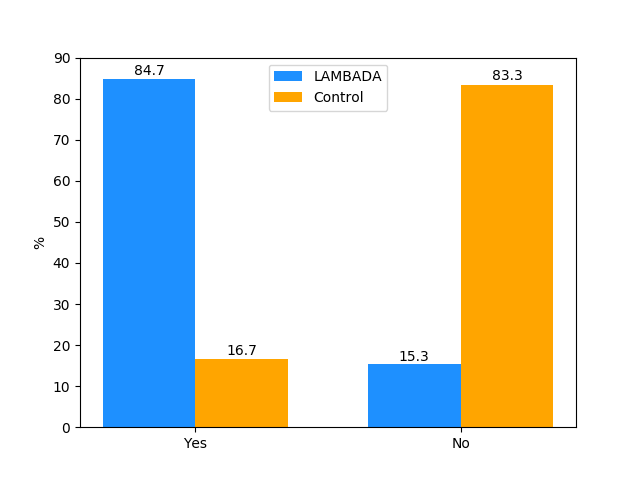
\includegraphics[scale=0.55]{lambadaContext}
	\captionof{figure}{Target word appears in passage.}
	\label{fig:lambadaContext}
\end{figure}

Indeed, in 84.7 \% of the LAMBADA items the target word (or its lemma, extracted with \texttt{nltk}'s WordNetLemmatizer) is mentioned in the context in the context, compared to the 15.3 \% for the control set. Furthermore, we can study the mention distance (understood as the number of words between the target word and its mention) distribution for LAMBADA. As illustrated in \autoref{fig:lambadaDistance}, 73 \% of the mentions are at a distance of more than 30 words (LAMBADA passages feature an average length of 75 words). This is specially important as many of the publicly available RNNLMs implementations are trained with TBPTT using a $k_2$ somewhere between 20 and 35.
 
\begin{figure}[H]
	\centering
	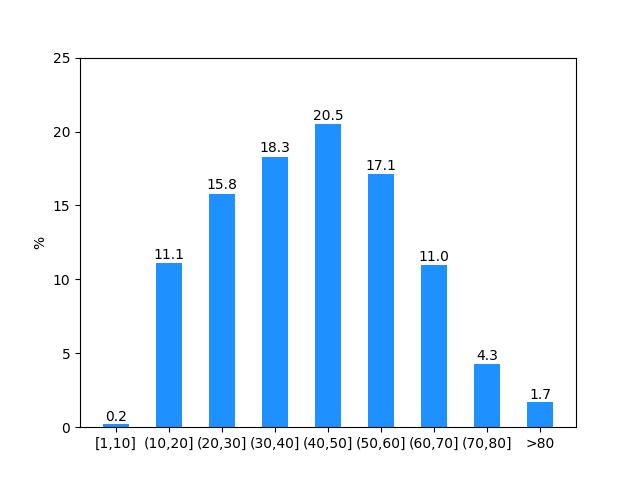
\includegraphics[scale=0.55]{lambadaDistance}
	\captionof{figure}{Target word appears in passage.}
	\label{fig:lambadaDistance}
\end{figure}

Moreover, it is also interesting to study the part of speech (PoS) tag distribution of the target words (also extracted with \texttt{nltk}'s default PoS tagger). As shown in \autoref{fig:lambadaPos}, proper nouns lead (48.1\%) followed by common nouns (37\%) and, far-off, verbs
(7.7\%). By comparing with control's PoS distribution, it is clear that proper nouns are over-represented in LAMBADA while the rest of the categories are downplayed.

\begin{figure}[H]
	\centering
	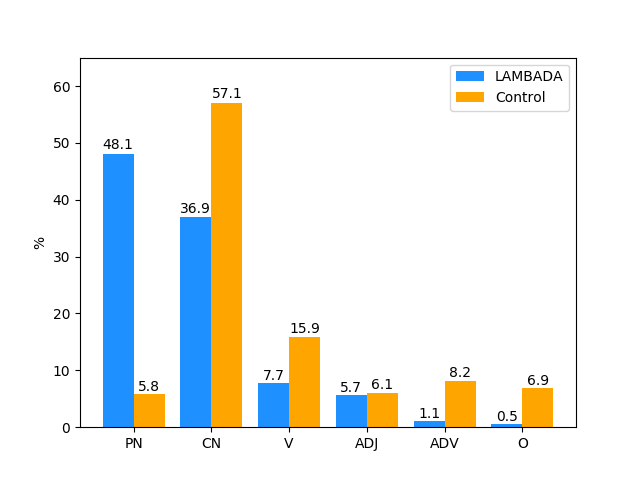
\includegraphics[scale=0.55]{lambadaPos}
	\captionof{figure}{Target words' PoS distribution (PN=proper noun, CN=common noun, V=verb, ADJ=adjective, ADV=adverb, O=other).}
	\label{fig:lambadaPos}
\end{figure}

\begin{figure}[H]
	\centering
	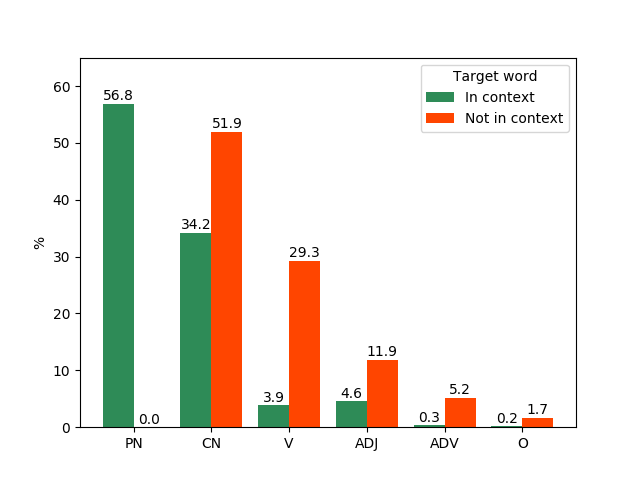
\includegraphics[scale=0.55]{lambadaPosAndContext}
	\captionof{figure}{LAMBADA target words' PoS distribution.}
	\label{fig:lambadaPosAndContext}
\end{figure}

The authors argue that the reason for this bias is the fact that proper nouns are favored by the specific setup. Namely, in many cases the context clearly demands a referential expression and the constraint of predicting a single word excludes other possibilities such as noun phrases with articles. This hypothesis seems to be confirmed by \autoref{fig:lambadaPosAndContext}, which shows the PoS distribution for LAMBADA split depending on whether the target word appears in the context. It can be seen that explicit mention in the preceding discourse context is critical for proper nouns (when the target word doesn't previously appear in the passage, none of them are proper nouns), while the other categories can often be guessed without having been explicitly introduced.

To sum up, we can conclude that LAMBADA does indeed put to the test language models' capabilities to exploit \textbf{long-range dependencies}. Besides, it is also important to note the bias towards proper nouns present in the dataset. Proper nouns are used to refer unique entities (e.g. the name of a specific character in a book) and due to their very nature, they are \textbf{rare words} (when compared to the rest of the training corpus). We will describe this phenomena in detail in the next section.

\section{The Rare Word Problem}
\label{sec:problemRare}

Talk about the well known problem of static language models and lack of adaptation -> cache models?

\cite{gulcehre2016pointing} describes the rare word problem with the vocab softmax and so on. Rare words won't generalize

\begin{figure}[H]
	\centering
	\begin{subfigure}{.5\textwidth}
		\centering
		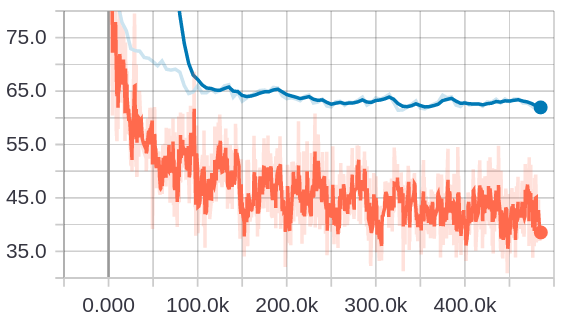
\includegraphics[scale=0.325]{perplexity_all}
		\caption{All words}
		\label{fig:perplexity_all}
	\end{subfigure}%
	\begin{subfigure}{.5\textwidth}
		\centering
		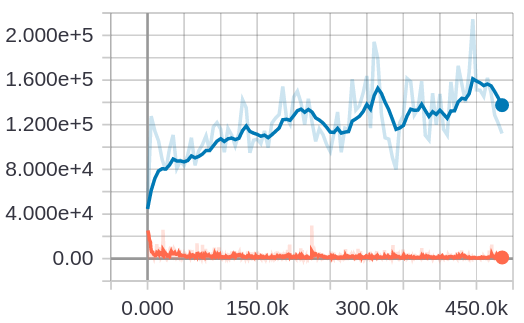
\includegraphics[scale=0.325]{perplexity_names}
		\caption{Only names}
		\label{fig:perplexity_names}
	\end{subfigure}
	\caption{Perplexity traces.}
	\label{fig:perplexity}
\end{figure}

\section{RNN Regularization}
\label{sec:rnnRegularization}

In this section we will describe in detail several modern techniques for regularizing recurrent neural networks:

\subsection{Dropout}

Start with original Dropout paper

\begin{figure}[H]
	\centering
	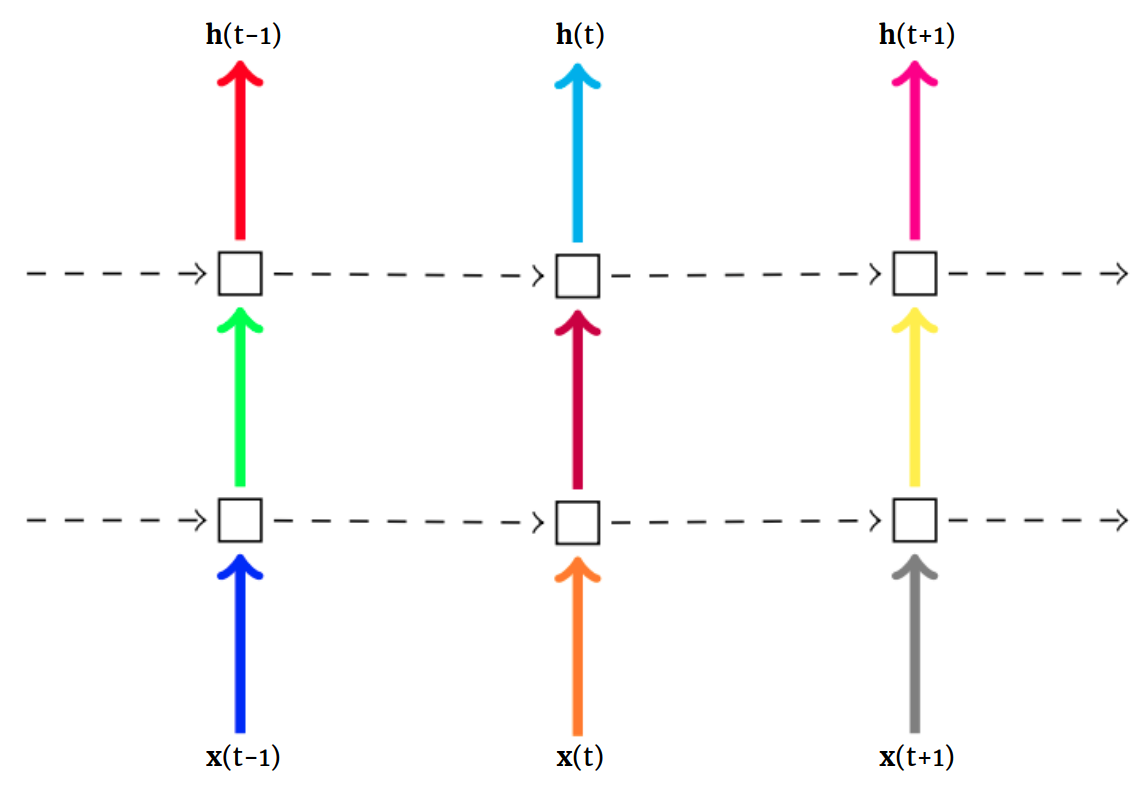
\includegraphics[scale=0.2]{dropout}
	\captionof{figure}{Naive Dropout \cite{gal2016theoretically}.}
	\label{fig:dropout}
\end{figure}

\subsection{Variational Dropout}

\begin{figure}[H]
	\centering
	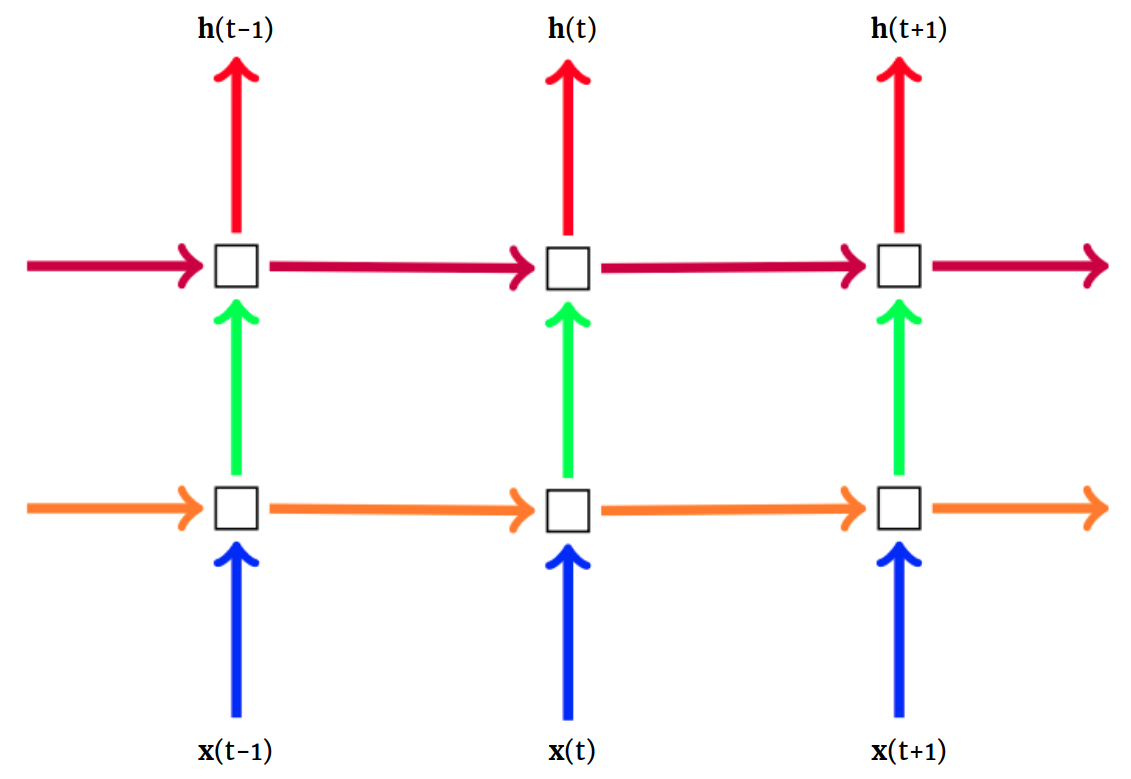
\includegraphics[scale=0.2]{varDropout}
	\captionof{figure}{Variational Dropout \cite{gal2016theoretically}.}
	\label{fig:varDropout}
\end{figure}

\subsection{Zoneout}

\subsection{Weight Dropout}
